\documentclass[
    11pt,
    a4paper,
    egregdoesnotlikesansseriftitles,
    toc=chapterentrywithdots,
    oneside,openright,
    titlepage,
    parskip=half,
    headings=normal,  % reduces heading size
    listof=totoc,
    bibliography=totoc,
    index=totoc,
    captions=tableheading,  % caption below table
    chapterprefix,
    listof=flat,
    final
]{scrbook}


% details about your thesis
\newcommand{\titel}{Conceptual design and realization of a graphical tool for determining the test coverage of digital circuit diagrams}
\newcommand{\artderarbeit}{Masterarbeit}  % {Bachelorarbeit,Masterarbeit}
\newcommand{\autor}{Razvan Matis}
\newcommand{\studiengang}{Softwareengineering und Informationstechnik}  % {Informatik,Wirtschaftsinformatik,Medieninformatik}
\newcommand{\matrikelnr}{2403005}
\newcommand{\erstgutachter}{Prof.\,Dr.~Flaviu Popp-Nowak}
\newcommand{\zweitgutachter}{Prof.\,Dr.~Claus Kuntzsch}
\newcommand{\betreuer}{Dr. \,~Kristian Trenkel}
\newcommand{\unternehmen}{ProMik GmbH}
\newcommand{\logo}{figures/TH-Nuernberg-RGB.png}
\newcommand{\keywords}{hot, fuzz}
 

% custom head and foot
\usepackage[automark]{scrlayer-scrpage}
\pagestyle{scrheadings}
\ihead{\headmark}
\chead{}
\ohead{\pagemark}
\renewcommand*\chaptermarkformat{\chapappifchapterprefix{\ }% 
  \thechapter.\enskip}

\RedeclareSectionCommand[tocindent=0pt]{section}
\RedeclareSectionCommand[tocindent=0pt]{subsection}
%\RedeclareSectionCommand[tocnumwidth=70pt]{chapter}

\usepackage{scrhack}

% other packages
\usepackage[square,sort,comma,numbers]{natbib}
\usepackage[utf8]{inputenc}
\usepackage[T1]{fontenc}
\usepackage{lmodern,relsize,textcomp,csquotes}
\usepackage{amsmath,amsfonts}
\usepackage[ngerman,english]{babel}  % flip for German thesis
\usepackage[final]{graphicx}
\usepackage{setspace,geometry,xcolor}
\usepackage{makeidx}
\usepackage{url}
\usepackage{paralist,ifthen,todonotes}
\usepackage{url}
\usepackage{hhline}
\usepackage{acronym}
\usepackage[toc]{glossaries}
\usepackage{pdfpages}

% table setup
\usepackage{longtable}
\usepackage{array}
\usepackage{ragged2e}
\usepackage{lscape}

% pdf hyperref
\usepackage[
    bookmarks=true,
    bookmarksopen=true,
    bookmarksnumbered=true,
    bookmarksopenlevel=1,
    pdftitle={\titel},
    pdfauthor={\autor},
    pdfcreator={\autor},
    pdfsubject={\titel},
    pdfkeywords={\keywords},
    pdfpagelabels=true,
    colorlinks=true,
    linkcolor=red,
    urlcolor=magenta,
    anchorcolor=black,
    citecolor=cyan,
    filecolor=magenta,
    menucolor=red,
    plainpages=false,
    hypertexnames=true,
    linktocpage=true,
]{hyperref}


% configure your listings style
\usepackage{listings}
\lstset{
	tabsize=3,
	extendedchars=true,
	frame=single,
	showstringspaces=true,
	numbers=left,
	numberstyle=\small,
	breakautoindent=true
}

\usepackage{protobuf/lang}  % include language definition for protobuf
\usepackage{protobuf/style} % include custom style for proto declarations.

% page setup
% \setlength{\topskip}{\ht\strutbox}
\geometry{paper=a4paper,left=2.5cm,top=3.0cm,bindingoffset=.8cm}
\onehalfspacing
\frenchspacing
\clubpenalty = 10000
\widowpenalty = 10000 
\displaywidowpenalty = 10000

% some commands
\newcommand{\ua}{\mbox{u.\,a.\ }}
\newcommand{\zB}{\mbox{z.\,B.\ }}
\newcommand{\dahe}{\mbox{d.\,h.,\ }}
\newcommand{\bzw}{\mbox{bzw.\ }}
\newcommand{\bzgl}{\mbox{bzgl.\ }}
\newcommand{\eg}{\mbox{e.\,g.\ }}
\newcommand{\ie}{\mbox{i.\,e.\ }}
\newcommand{\wrt}{\mbox{w.\,r.\,t.\ }}
\newcommand{\etal}{\mbox{\emph{et.\,al.\ }}}


% TODO remove if not needed...
\usepackage{blindtext}

% load glossary entries
\makenoidxglossaries
\loadglsentries{glossary}

\definecolor{eclipseStrings}{RGB}{42,0.0,255}
\definecolor{eclipseKeywords}{RGB}{127,0,85}
\colorlet{numb}{magenta!60!black}

\lstdefinelanguage{json}{
    basicstyle=\normalfont\ttfamily,
    commentstyle=\color{eclipseStrings}, % style of comment
    stringstyle=\color{eclipseKeywords}, % style of strings
    numbers=left,
    numberstyle=\scriptsize,
    stepnumber=1,
    numbersep=8pt,
    showstringspaces=false,
    breaklines=true,
    frame=lines,
    backgroundcolor=\color{white}, %only if you like
    string=[s]{"}{"},
    comment=[l]{:\ "},
    morecomment=[l]{:"},
    literate=
        *{0}{{{\color{numb}0}}}{1}
         {1}{{{\color{numb}1}}}{1}
         {2}{{{\color{numb}2}}}{1}
         {3}{{{\color{numb}3}}}{1}
         {4}{{{\color{numb}4}}}{1}
         {5}{{{\color{numb}5}}}{1}
         {6}{{{\color{numb}6}}}{1}
         {7}{{{\color{numb}7}}}{1}
         {8}{{{\color{numb}8}}}{1}
         {9}{{{\color{numb}9}}}{1}
}


\begin{document}
\setcounter{secnumdepth}{3}  % numerate subsections
\setcounter{tocdepth}{2}  % ...but don't include them in toc

\frontmatter
\include{cover}\cleardoublepage

% download the following form and complete it (hit save in your editor)
% https://intern.ohmportal.de/fileadmin/Gelenkte_Doks/Abt/SZS/SB/SB_0050_FO_Pruefungsrechtliche_Erklaerung_und_Erklaerung_zur_Veroeffentlichung_der_Abschlussarbeit_public.pdf
% \includepdf{SB_0050_FO_Pruefungsrechtliche_Erklaerung_und_Erklaerung_zur_Veroeffentlichung_der_Abschlussarbeit_public.pdf}\cleardoublepage

\chapter{Abstract}
According to \ac{PCB}s and their digital circuits which are getting more complex all the time there is the requirement of being able to determine the test coverage of it. In dependency on these determined values then automatic boundary scan test chains could be performed or the need of changing something on the layout will be visible. This thesis describes the way of the conceptual design and the realization of a graphical tool for loading, showing different digital circuit diagrams projects which need to be in the \ac{ODB}++ format and the determination of test coverage parameters as well as the creation of \ac{SVF} files for being able to run the boundary scan test chains on these special devices which contains at least one \ac{JTAG} device. Furthermore there will be described detailed information about the frameworks, programming patterns and best practices which were used for creating this \ac{MVVM} C\# project and the project structure itself which was created for making sure to have the following key features available:
\begin{itemize}
	\item Opening any \ac{ODB}++ project by connecting to a stand alone \ac{GRPC} server and using the \ac{PCB}-Investigator API
	\item Exporting any opened projects to \ac{JSON} file for later usage and importing of that created files
	\item Creation and loading of project files which contains a manifest file for information about the project structure itself
	\item Modifying, exporting and importing of different kind of settings according the connection to the \ac{GRPC} server, the appearance and the test coverage values
	\item Determination of different test coverage values according to the boundary scan mechanism
	\item Creation of \ac{SVF} files for run the boundary scan test chain with a programmer from ProMik GmbH on a \ac{JTAG} containing device
\end{itemize}

\tableofcontents

\mainmatter
\chapter{List of abbreviations}

\begin{acronym}[Bash]
 \acro{MES}{manufactoring execution system}
 \acro{SAP}{semi-automated production programming station}
\end{acronym}

\chapter{Introduction}

	\section{Motivation}

	\section{Requirements}

	\section{Programming language and operating system}
\chapter{Fundamentals}

	\section{PCB Investigator}

	\section{ODB++ project format}

	\section{JTAG device}

	\section{Boundary scan}

	\section{SVF file format}

	\section{GRPC}

	\section{JSON format}
\chapter{Conceptual design}
First of all the structure itself of the received objects needs to be analyzed more in detail which are being provided by the \textbf{PCB-Investigator.exe}:\\

\begin{figure}[h]
	\centering
		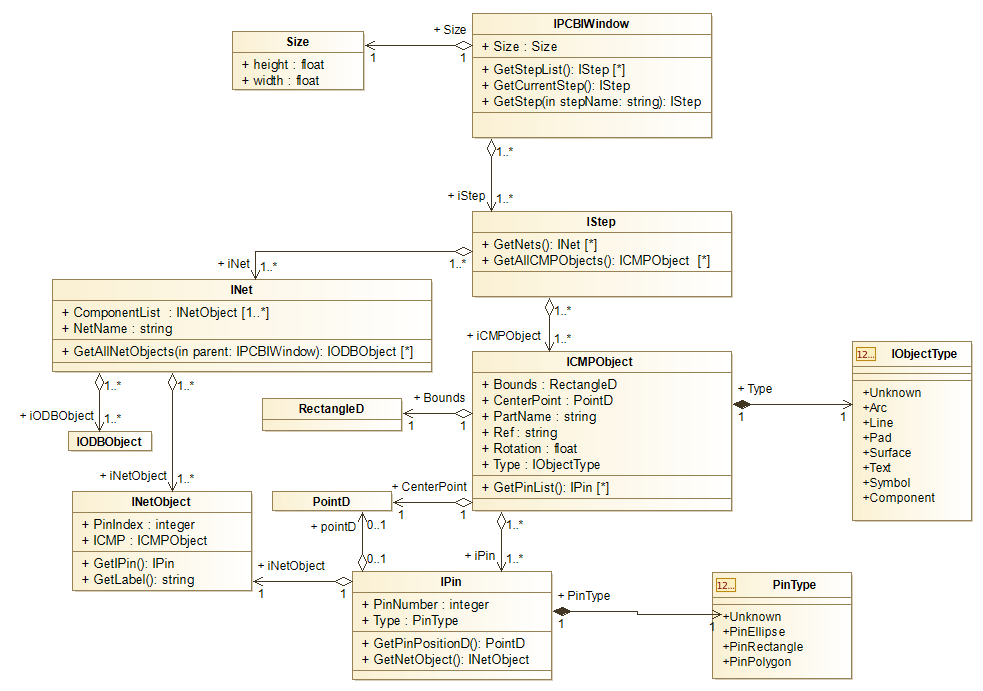
\includegraphics[width=1.00\textwidth]{figures/PCB Investigator class diagram.png}
	\caption{Class diagram of the PCB-Investigator objects of interest}
	\label{fig:PCB Investigator class diagram}
\end{figure}
As shown within \ref{fig:PCB Investigator class diagram} there could be seen that the very first class is the IPCBIWindow which contains a various amount of IStep objects. Within this IStep objects there are many INet objects and ICMPObjects. \newline
As ProMik GmbH is just interested in extracting all relevant information from any \ac{ODB}++ related projects the following public functions of the \textbf{PCB-Investigator.exe} where used by the created software\cite{.472021b} to extract all INet and ICMPObjects:

\begin{itemize}
	\item IAutomation.IAutomationInit() - Initialization of the \ac{API}
	\item IAutomation.CreateNewPCBIWindow(bool visible) - Creates the base window
	\item IPCBIWindow.LoadData(string path) - Loads a specific project into the window
	\item IPCBIWindow.GetStepList() - Getter for all steps of the window
	\item IStep.GetNets() - Getter for all nets of a step
	\item IStep.GetAllLayerNames() - Getter for all layer names of a step
	\item IStep.GetLayer(string layerName) - Getter for a layer in dependency on the layer name from a step
	\item ILayer.GetAllLayerObjects() - Getter for all objects which are located on a specific layer within a step
\end{itemize}
\chapter{Architecture}
Within this chapter the architecture of the implemented software will be described in detail according to the used project structure of the visual studio solution.
	\section{Overview}
	
\begin{center}
	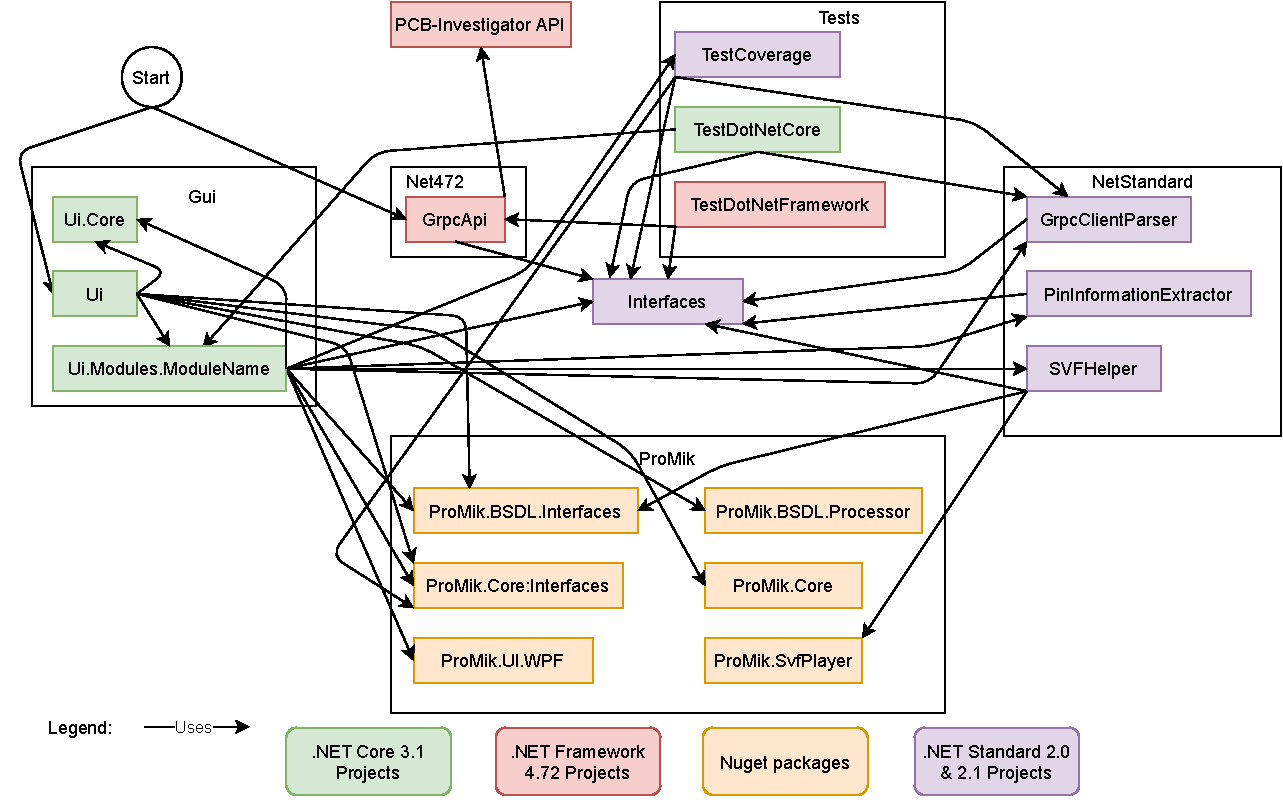
\includegraphics[width=1.00\textwidth]{figures/project structure.pdf}
	\begin{figure}[!h]
	\caption{Project overview}
	\label{fig:projectOverview}
	\end{figure}
\end{center}

As shown in \ref{fig:projectOverview} it will be clear that the whole project is organized in different kind of folders which contain C\# projects. On one side there is the \textbf{Gui} folder containing the following projects:
\begin{itemize}
	\item Ui.Core - This project contains the region names and the view model bases which should be inherited and was provided by the PRISM framework.
	\item Ui - Within the project the mainView and mainViewModel could be found (Was initially created by the PRISM framework)
	\item Ui.Modules.ModuleName - This project was basically created by the PRISM framework and contains all necessary events, interfaces, models, viewmodels and views for operating with all other referenced projects
\end{itemize}
On the other side there is the \textbf{Net472} folder with the project GrpcApi which contains the standalone software for referencing the \ac{PCB}-Investigator API and runs as a \ac{GRPC} server. Next the \textbf{NetStandard} folder contains the following projects:
\begin{itemize}
	\item GrpcClientParser - The \ac{GRPC} client project for communicating with the GrpcApi project for getting all parsed objects by the \ac{PCB}-Investigator API
	\item PinInformationExtractor - This project is being used for creation of textfiles in \ac{JSON} format containing all pin information of all \ac{JTAG} devices of one project.
	\item SVFHelper - This project is needed for creation of \ac{SVF} files in dependency on \ac{BSDL} files which should be referenced for \ac{JTAG} devices. Further it could play \ac{SVF} files with a programmer from ProMik which is connected to a boundary scan compatible \ac{JTAG} device
\end{itemize}
The \textbf{Tests} folder consists of the following projects:
\begin{itemize}
	\item TestCoverage - This project contains all boundary scan test according logic to be performed
	\item TestDotNetCore - Here there can be found different unit tests for the parser logic of the GrpcClientParser project
	\item TestDotNetFramework - This project contains unit tests to be performed using the GrpcApi project
\end{itemize}
Finally there were different \textbf{ProMik} related projects included by the nuget package manager of visual studio:
\begin{itemize}
	\item ProMik.BSDL.Interfaces - Contains all interfaces regarding the BSDL handling
	\item ProMik.BSDL-Processor - Contains the implementations regarding the BSDL processor
	\item ProMik.Core.Interfaces - The interfaces of core logic
	\item ProMik.Core - The implementations of core logic
	\item ProMik.UI.WPF - Contains different Ui elements which could be included (settings panel, logPanel \ac{etc.})
	\item ProMik.SvfPlayer - Contains the logic for creation and playing of \ac{SVF} files
\end{itemize}

	\section{Interfaces}
The Interfaces project was created as a .NET standart 2.0 project to make sure it could be referenced by any other projects which needs it. It has the following content:
\begin{itemize}
	\item Gui - Within this folder are just interfaces located which are related to the Gui logic
	\begin{itemize}
		\item IDialogSelector - It could be used for the handling of dialogs which should be shown either for file opening, saving or folder opening or saving
		\item ILogger - The system wide used interface for logging purposes which additionally will be written into a local logfile
	\end{itemize}
	\item Helper - A folder wich contains objects which were necessary for the two unit test related projects
	\begin{itemize}
		\item PcbTestObject - This is a helper class for unit test purposes
		\item PinTestObject - It is a helper class which is been included in the PcbTestObjects class and provides more detailed pin information
	\end{itemize}
	\item PcbInvestigator - That folder contains all \ac{PCB}-Investigator related interfaces and their implementations of the received objects
	\begin{itemize}
		\item IFunctionalAttributes - The interface which contains all functional related attributes
		\item IGeometricAttributes - A interface which contains all geometric and position related information
		\item INetComponent - This is the interface for representing a net object
		\item IPinComponent - That is a interface for describing a pin object
		\item IPCBComponent - An interface which contains all information about a PCBComponent
		\item Enums - Within that folder are the enumerations placed which were used within the IPCBComponent and IPinComponent for defining the componentType and pinType
		\item Implementations - In that folder are all implementations of the predefined interfaces of the PCBInvestigator objects located
	\end{itemize}
\end{itemize}

	\section{Grpc Server for using the PCB Investigator API}
This project is responsible for using the \ac{PCB}-Investigator API which is being created using the .NET Framework and was created as a console application using the .NET Framework 4.72 as well. It further derives a service which was provided by a \ac{GRPC} auto code generation as a server. The proto file itself which was used for the code generation contains three functions:
\begin{itemize}
	\item GetConvertedObjects(Request) returns (Result) - Within this function all objects of a specific project could be determined using the location to the project
	\item GetConvertedObjectsByZip(RequestZip) returns (Result) - That method obtains all objects by using the received project as zip file in bytes
	\item ClientAvailable(Empty) returns (StatusResult) - This function is being used to detect whether the client has a valid connection to the server using the settings or not
\end{itemize}

	\section{Grpc Client for connecting to the Server and parsing all objects}

	\section{GUI}

		\subsection{Events}

		\subsection{Helper}

		\subsection{Interfaces}

		\subsection{Implementations}

		\subsection{Model}

		\subsection{ViewModels}

		\subsection{Views}

		\subsection{MainView and MainViewModel}

	\section{Test coverage determination of loaded project}

	\section{Pin information extraction}

	\section{SVF file generator}

	\section{Unit tests}
\chapter{Analysis}

	\section{Performance of loading ODB++ projects by using the PCBInvestigator API}

	\section{Performance of loading projects by importing JSON formatted files}

	\section{Performance of exporting projects into JSON format}

	\section{Performance of showing connections of components}

	\section{Performance of determination of test coverage values}
\chapter{Conclusion}
As a conclusion of the creation of the requested tool there could be definitely held that in dependency on all requirements which were communicated by ProMik GmbH and the software developer a quit powerful and feature rich software was provided according to \ref{fig:projectOverview}. All at the beginning requested requirements from \ref{items:req} were successfully implemented. Further there were provided the following features as bonus content:
\begin{itemize}
	\item Mirroring of the whole rendered project across the x and y axis is possible
	\item Defining of steps to be considered at read out from \ac{PCB}-Investigator could be defined within settings
	\item Coloring of all components independently is possible by changing the settings
	\item An coordinates origin is being placed
	\item The actual mouse position is being shown at the bottom of the tool by providing the x and y coordinate
\end{itemize}

As potential extensions or improvements there could be considered the following point in the view of the developer:
\begin{itemize}
	\item Inclusion of \ac{SVF} player for being able to perform \ac{SVF} files by the tool directly
	\item Tracing of the \ac{SVF} results (comparison between TDI and TDO values) and detailed logging about the detected differences
	\item Usage of other API for gathering information from \ac{ODB}++ related projects than just the \ac{PCB}-Investigator
	\item Provide drag \& drop possibility of rendered components for being able to classify directly as blacklist component for the test coverage determination
	\item Provide more test coverage determination methods than just the boundary scan ones
	\item Usage of decryption \& encryption of exported data files to avoid manipulation of it
\end{itemize}

At the beginning already the need was discussed to be able to work with that whole created project as comfortable as possible for being able to integrate such extensions. The developer is of the opinion that especially by usage of all requested frameworks, patterns and integration of as much interfaces as possible this requirement was satisfied. Further there were kept a highly structured way of creation of different independent projects which leads to the possibility of using them stand alone or even as a nuget package within the intranet of the company.
\chapter{Credits}
Within this small chapter I would like to thank a couple of people who made this work possible by supporting me in many different areas of my life. \newline
First of all I want to thank my parents \textbf{Gabriela} and \textbf{Nicolae Matis} who have born, raised and supported me in every single minute of my life. I know I unfortunately didn't
always make you proud of my actions but I hope that I am still working on it successfully by milestones like this one. Mum I really hope for you that you will
solve your physical constraints successfully and dad I hope that you stay as young as you are for a really long time \newline

Afterward I would like to thank my brother \textbf{Nik Matis} and my sister \textbf{Michelle Matis} who have supported me in that way as a brother just could expect it to be perfect. 
Michelle I wish you all the best with your study and Nik I hope you will find your destiny in choosing a new job soon. \newline

And finally I would like to thank a couple of my best friends who have supported me in investing much free time with myself and were successfully responsible for
being able to forget all the stress about the work and enjoy my life. \newline

\textbf{Andreas Korkenländer} I already know you now about for 20 years and really hope that this will continue until my death. I wish you all the best with your new job and your intention of traveling around the world. \newline
\textbf{Dominik Müller} you were my first best friend after I moved to Nürnberg and I really hope that connection persists for a longer time although you are sometimes really a hardheaded person :) I wish you all the best with your new challenge of doing a new apprenticeship. \newline
\textbf{Rene Biedermann} you are one of that guys I'm able to speak about philosophic and esoteric topics and of course medical topics about my own health in a detailed way as I'm really impressed of it. I wish you all the best in accomplishing your exam for being an alternative practitioner and I really think that this will satisfy your life in complete way. \newline
\textbf{Willi Fritz} I would really like to thank you especially for the last year where you permitted me to do my training within your own flat and visited me almost every weekend for just hanging around and playing PlayStation 4 or for cooking some real tasty meals. I wish you all the best at finishing your tax consultant state examination and am really looking forward of traveling around the world with your person soon.

% remove if not needed
\appendix
\chapter{User manual for working with the smart Inter Circuit Tests (ICT) analyzer tool}
This document describes the way of handling the tool for determining the test coverage of different \ac{ODB}++ related projects.
\section{Overview}

\begin{center}
	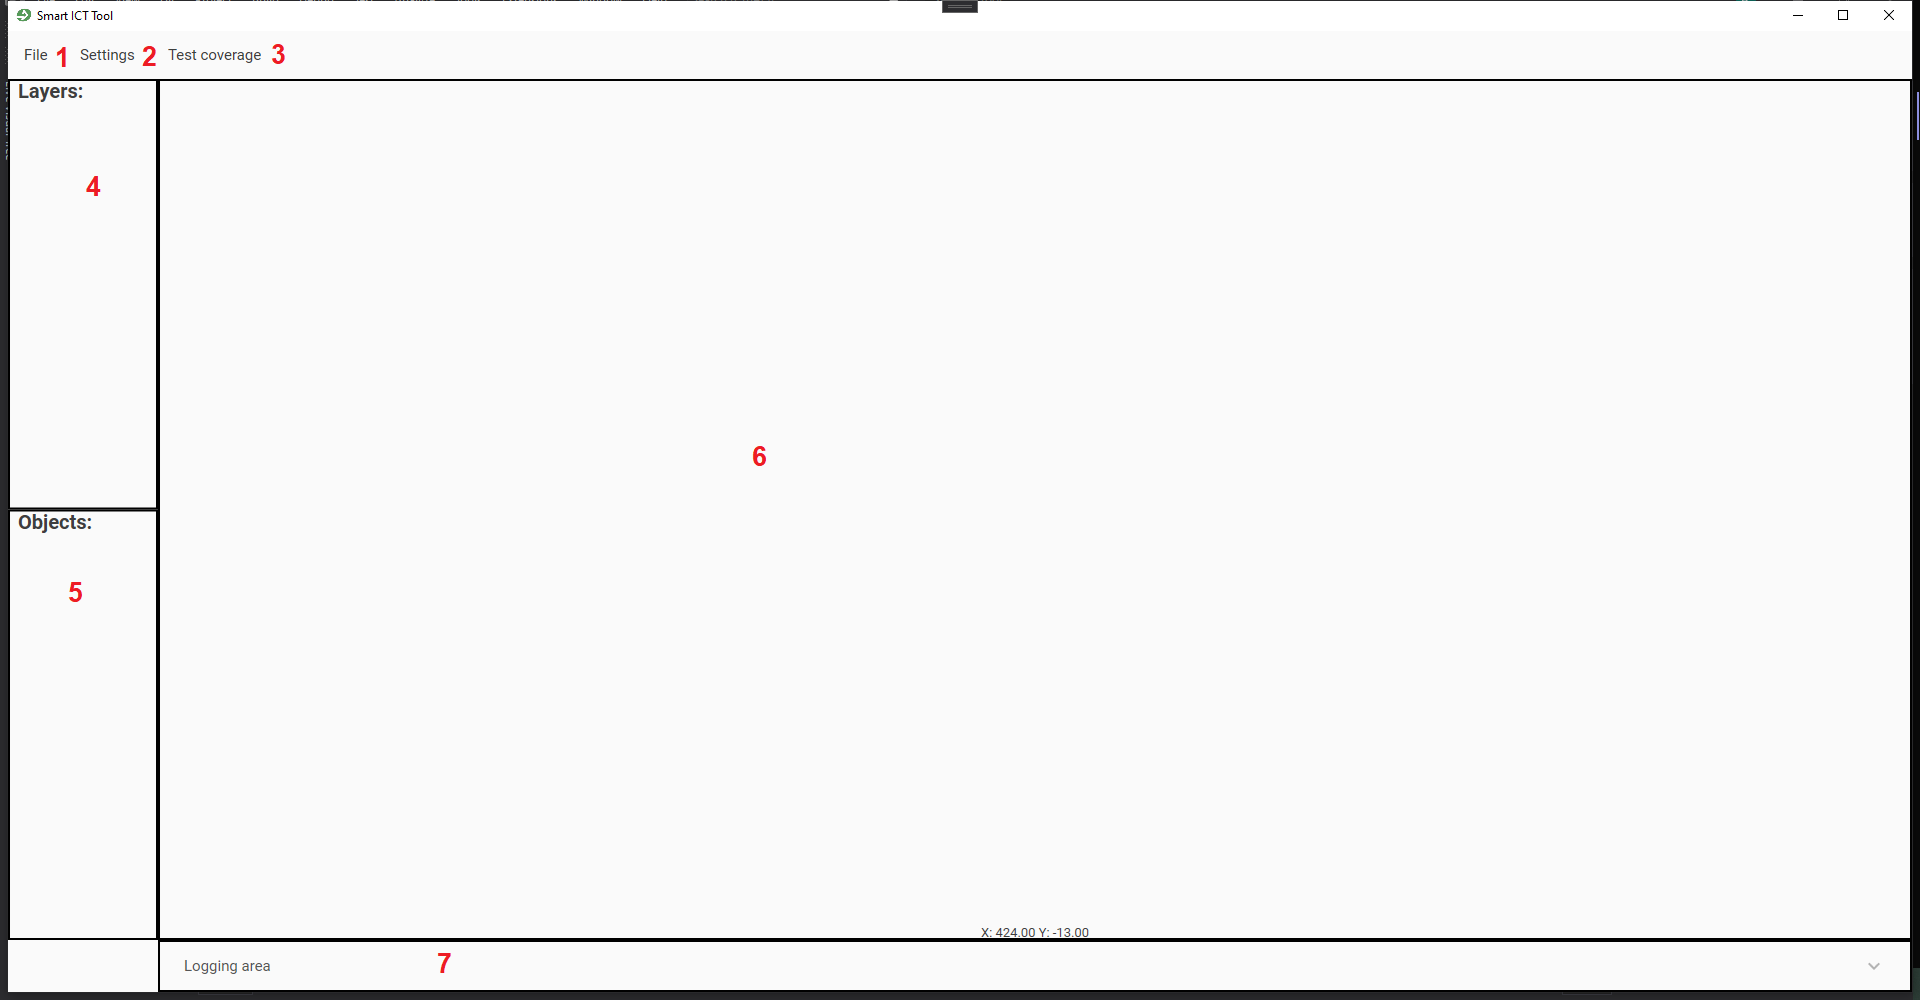
\includegraphics[width=1.00\textwidth]{figures/attachments/overview.png}
	\begin{figure}[!h]
	\caption{Tool overview}
	\label{fig:Tooloverview}
	\end{figure}
\end{center}

As shown in \ref{fig:Tooloverview} the tool itself consists of seven different areas of interest:
\begin{enumerate}
	\item File menu group - performing actions regarding the opening of project files, ...
	\item Settings - selection of settings, importing and exporting them
	\item Test coverage - all test coverage related actions
	\item Layers - the layers overview
	\item Objects - the test coverage objects list
	\item the rendered component view
	\item The logging area
\end{enumerate}

\section{Settings}

\begin{center}
	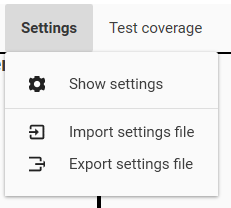
\includegraphics[scale=0.60]{figures/attachments/settingsOverview.png}
	\begin{figure}[!h]
	\caption{Settings overview}
	\label{fig:Settingsoverview}
	\end{figure}
\end{center}

As shown in \ref{fig:Settingsoverview} there are the following three menu items available:
\begin{enumerate}
	\item Show settings - opens the settings page for all settings
	\item Import settings file - a file chooser will pop up for selecting a settings database file to be imported
	\item Export settings file - a file chooser will pop up for selecting the target file where the settings database should be exported to
\end{enumerate}

\subsection{Show settings}
After clicking on the menu item All settings a new window will be shown containing all setting pages.
\subsubsection{PCB Investigator \ac{API} settings}

\begin{center}
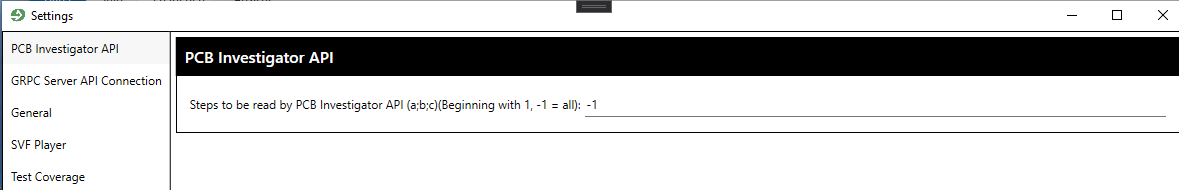
\includegraphics[width=1.00\textwidth]{figures/attachments/pcbInvestigatorSettings.png}
	\begin{figure}[!h]
	\caption{PCB Investigator \ac{API} settings}
	\label{fig:pcbInvestigatorSettings}
	\end{figure}
\end{center}

As shown in \ref{fig:pcbInvestigatorSettings} there is the possibility of changing the steps which should be considered for read out from the \ac{API}. -1 means all steps should be read out. Other values could be defined semicolon separated

\subsubsection{GRPC server \ac{API} connection settings}

\begin{center}
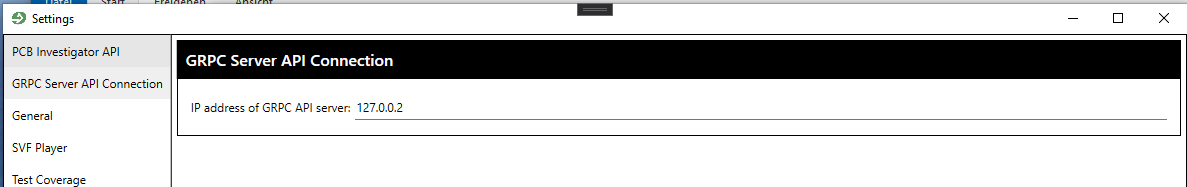
\includegraphics[width=1.00\textwidth]{figures/attachments/grpcServerSettings.png}
	\begin{figure}[!h]
	\caption{\ac{GRPC} server \ac{API} connection settings}
	\label{fig:grpcServerSettings}
	\end{figure}
\end{center}

As shown in \ref{fig:grpcServerSettings} there is the possibilty of changing the ip address of the \ac{GRPC} server to connect to

\subsubsection{General settings}

\begin{center}
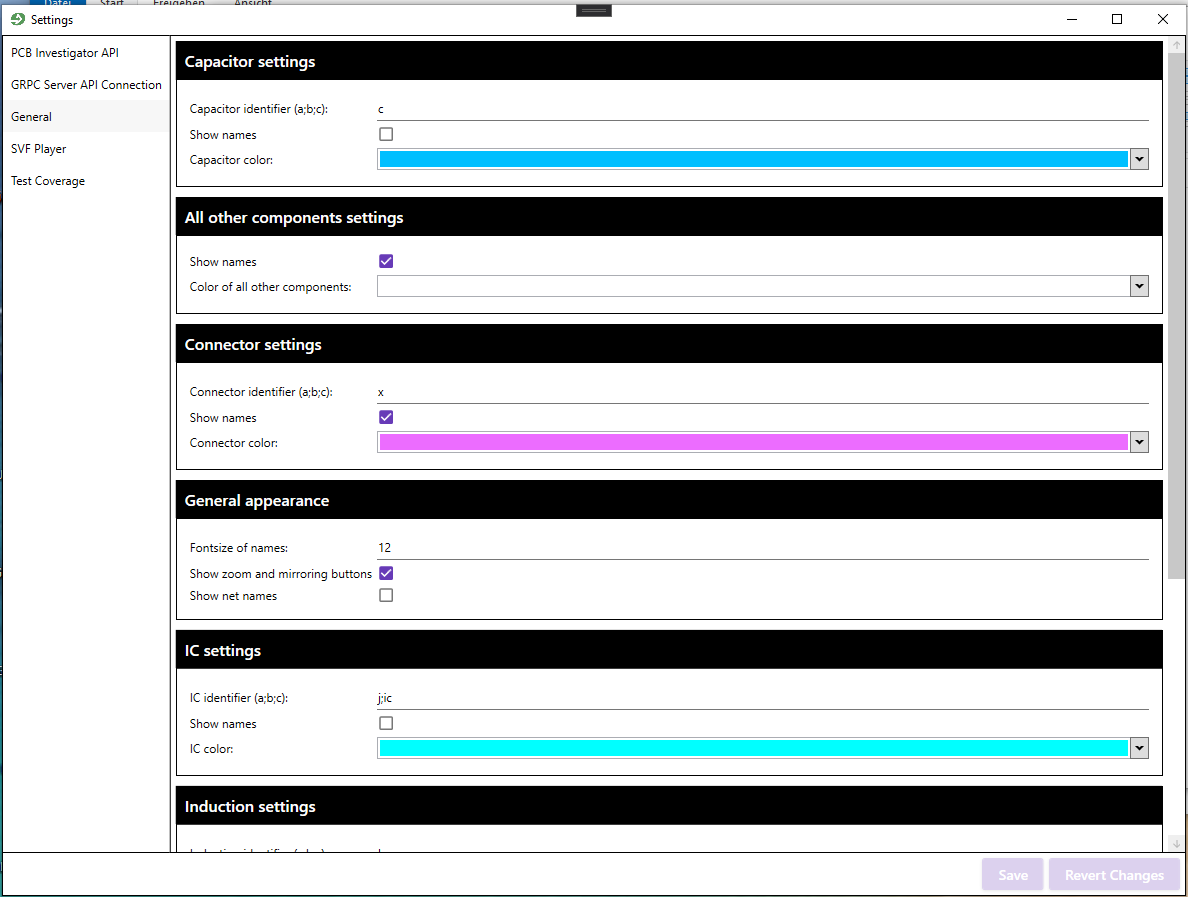
\includegraphics[width=1.00\textwidth]{figures/attachments/generalSettings1.png}
	\begin{figure}[!h]
	\caption{General settings 1}
	\label{fig:generalSettings1}
	\end{figure}
\end{center}

Within the first part of the general settings (\ref{fig:generalSettings1}) there are the following settings available (identifier, show names and the color):
\begin{itemize}
	\item Capacitor
	\item Other components
	\item Connector
	\item \ac{IC}
\end{itemize}
Fruthermore there are the following settings available:
\begin{itemize}
	\item General appearance
	\begin{itemize}
		\item Fontsize of names
		\item Show zoom and mirroring buttons
		\item Show net names
	\end{itemize}
\end{itemize}

\begin{center}
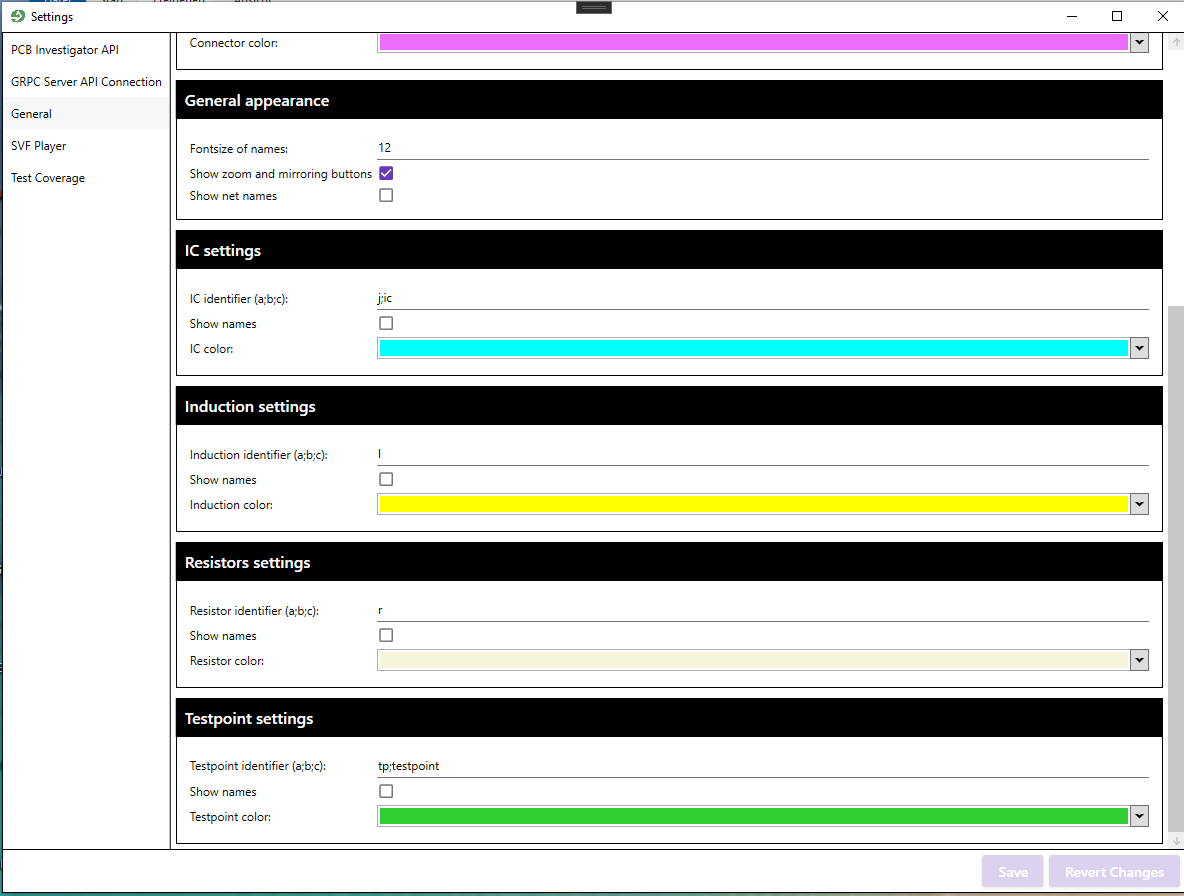
\includegraphics[width=1.00\textwidth]{figures/attachments/generalSettings2.png}
	\begin{figure}[!h]
	\caption{General settings 2}
	\label{fig:generalSettings2}
	\end{figure}
\end{center}

Within the second part of the general settings (\ref{fig:generalSettings2}) there are the following settings available (identifier, show names and the color):
\begin{itemize}
	\item Inductor
	\item Resistor
	\item Testpoint
\end{itemize}

\subsubsection{SVF Player settings}

\begin{center}
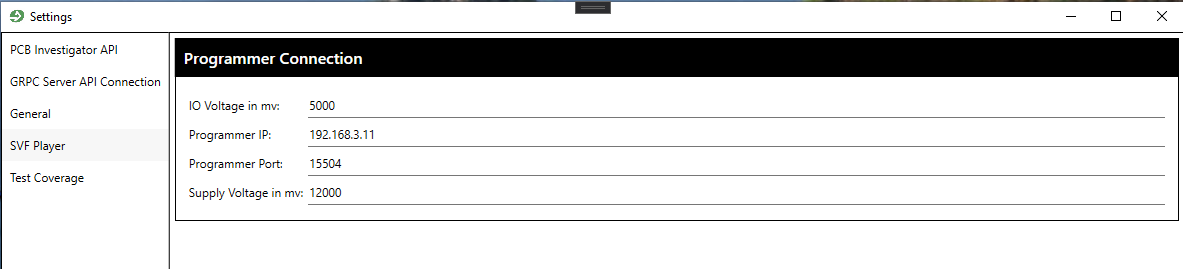
\includegraphics[width=1.00\textwidth]{figures/attachments/svfPlayerSettings.png}
	\begin{figure}[!h]
	\caption{\ac{SVF} Player settings}
	\label{fig:svfPlayerSettings}
	\end{figure}
\end{center}

As shown in \ref{fig:svfPlayerSettings} there are the following settings available:
\begin{itemize}
	\item IO Voltage in mv
	\item Programmer IP
	\item Programmer Port
	\item Supply Voltage in mv
\end{itemize}

\subsubsection{Test Coverage settings}

\begin{center}
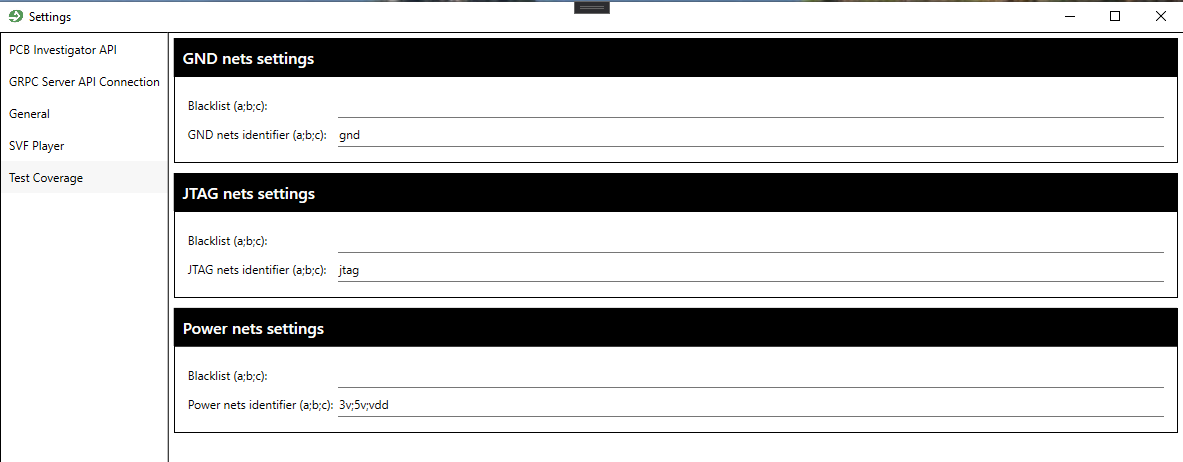
\includegraphics[width=1.00\textwidth]{figures/attachments/testCoverageSettings.png}
	\begin{figure}[!h]
	\caption{Test Coverage settings}
	\label{fig:testCoverageSettings}
	\end{figure}
\end{center}

As shown in \ref{fig:testCoverageSettings} there are the following settings available (blacklist of nets and net identifier):
\begin{itemize}
	\item Ground
	\item \ac{JTAG}
	\item Power
\end{itemize}
Further more there is the possibility of defining the \ac{JTAG} pin identifier for making sure being able to use not just the default values \textbf{TMS, TDI, TDO, TCK}. That means in detail for correctly determining a \ac{JTAG} device there should be the following requirements accomplished:
\begin{enumerate}
	\item Set up the \textbf{\ac{IC} identifier} setting from general settings in that way that the \ac{JTAG} device is being recognized correctly as an \ac{IC} component
	\item Set up the \textbf{\ac{JTAG} nets identifier} from the test coverage settings in that way that the \ac{JTAG} device is correctly being recognized within a corresponding net
	\item Set up the \textbf{\ac{JTAG} pin identifier} setting from the test coverage settings in that way that the \ac{JTAG} device is correctly being recognized by its pins
\end{enumerate}

\subsection{Import / Export settings file}
By clicking on one of the menu items Settings -> Import settings file or Settings -> Export settings file afterward a new file selection dialog will be shown where to select the source / target file to be imported / exported. Further if the project file handling is enabled the settings file will automatically be stored within the project file and be loaded automatically on next opening of project file

\section{Project file}

\begin{center}
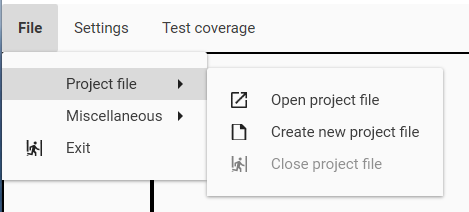
\includegraphics[scale=0.60]{figures/attachments/projectFile.png}
	\begin{figure}[!h]
	\caption{Project file handling}
	\label{fig:projectFile}
	\end{figure}
\end{center}

As shown in \ref{fig:projectFile} there is the possibility of choosing the following menu items within the File -> Project file group:
\begin{itemize}
	\item Open project file
	\item Create new project file
\end{itemize}

\section{Miscellaneous}

\begin{center}
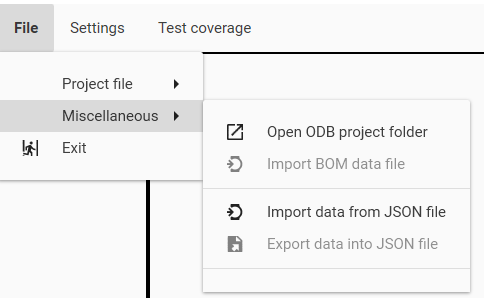
\includegraphics[scale=0.60]{figures/attachments/fileMisc.png}
	\begin{figure}[!h]
	\caption{Miscellaneous menu items}
	\label{fig:fileMisc}
	\end{figure}
\end{center}

As shown in \ref{fig:fileMisc} there are the following menu items available at File -> Miscellaneous:
\begin{itemize}
	\item Open \ac{ODB} project folder - after choosing that action a new dialog appears to select the folder which should be transferred to the \ac{GRPC} server as zipped content for read out by using the PCB-Investigator \ac{API}
	\item Import \ac{BOM} data file - After any project was successfully loaded then the import of a valid bill of materials file will be available. After choosing this a new window appears where to set up all relevant settings for import
	\item Import data from \ac{JSON} file - a new dialog appears where you are able to select any \ac{JSON} formatted file containing previously exported data of this application
	\item Export data into \ac{JSON} file - after any project was loaded successfully then this item will be accessible. After choosing it a new dialog appears where you could select the target for creation of a valid \ac{JSON} formatted file containing all data
\end{itemize}

\section{Creation of new project}
To create a new project just first click on File -> Project file -> Create new project file. After ward there will be a dialog shown for selecting the target file to be saved at:

\begin{center}
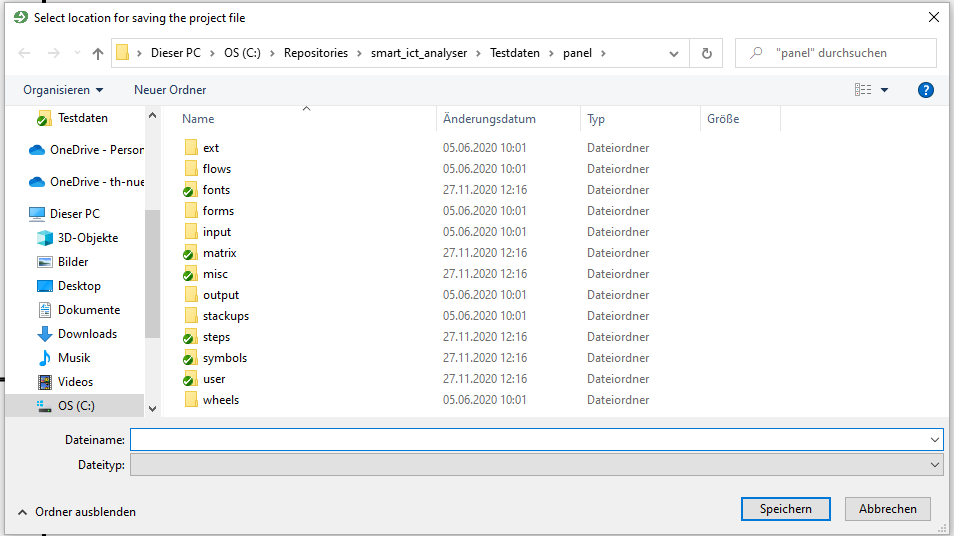
\includegraphics[scale=0.60]{figures/attachments/projectFileCreationDialog.png}
	\begin{figure}[!h]
	\caption{Project file creation dialog}
	\label{fig:projectFileCreationDialog}
	\end{figure}
\end{center}

After you confirmed your target within the dialog (\ref{fig:projectFileCreationDialog}) then you could proceed to open a new project. For that make sure to have a valid connection to the \ac{GRPC} server and click then File -> Miscellaneous -> Open \ac{ODB} project folder. After you chose a program during the communication and parsing from the \ac{GRPC} server there will be shown an animation:

\begin{center}
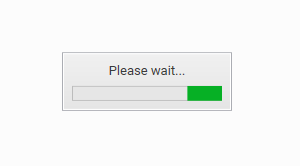
\includegraphics[scale=0.60]{figures/attachments/pleaseWait.png}
	\begin{figure}[!h]
	\caption{Please wait animation}
	\label{fig:pleaseWait}
	\end{figure}
\end{center}

After the process finished then if no values are defined for that components received a new dialog should be visible where to select the \ac{BOM} file for importing:

\begin{center}
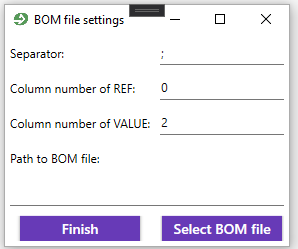
\includegraphics[scale=0.60]{figures/attachments/selectBom.png}
	\begin{figure}[!h]
	\caption{Select \ac{BOM} file dialog}
	\label{fig:selectBom}
	\end{figure}
\end{center}

After you set up the settings:
\begin{itemize}
	\item Separator
	\item Column number of REF
	\item Column number of VALUE
	\item Path to \ac{BOM} file - could be set by clicking on Select \ac{BOM} file where then a new dialog for selecting any file will be opened
\end{itemize}

within that dialog and selected a valid \ac{CSV} file to be imported then proceed by clicking on finish. \newline

After the process finished then on within the layers list there should be some layers available and the control buttons at the right bottom place will be visible:

\begin{center}
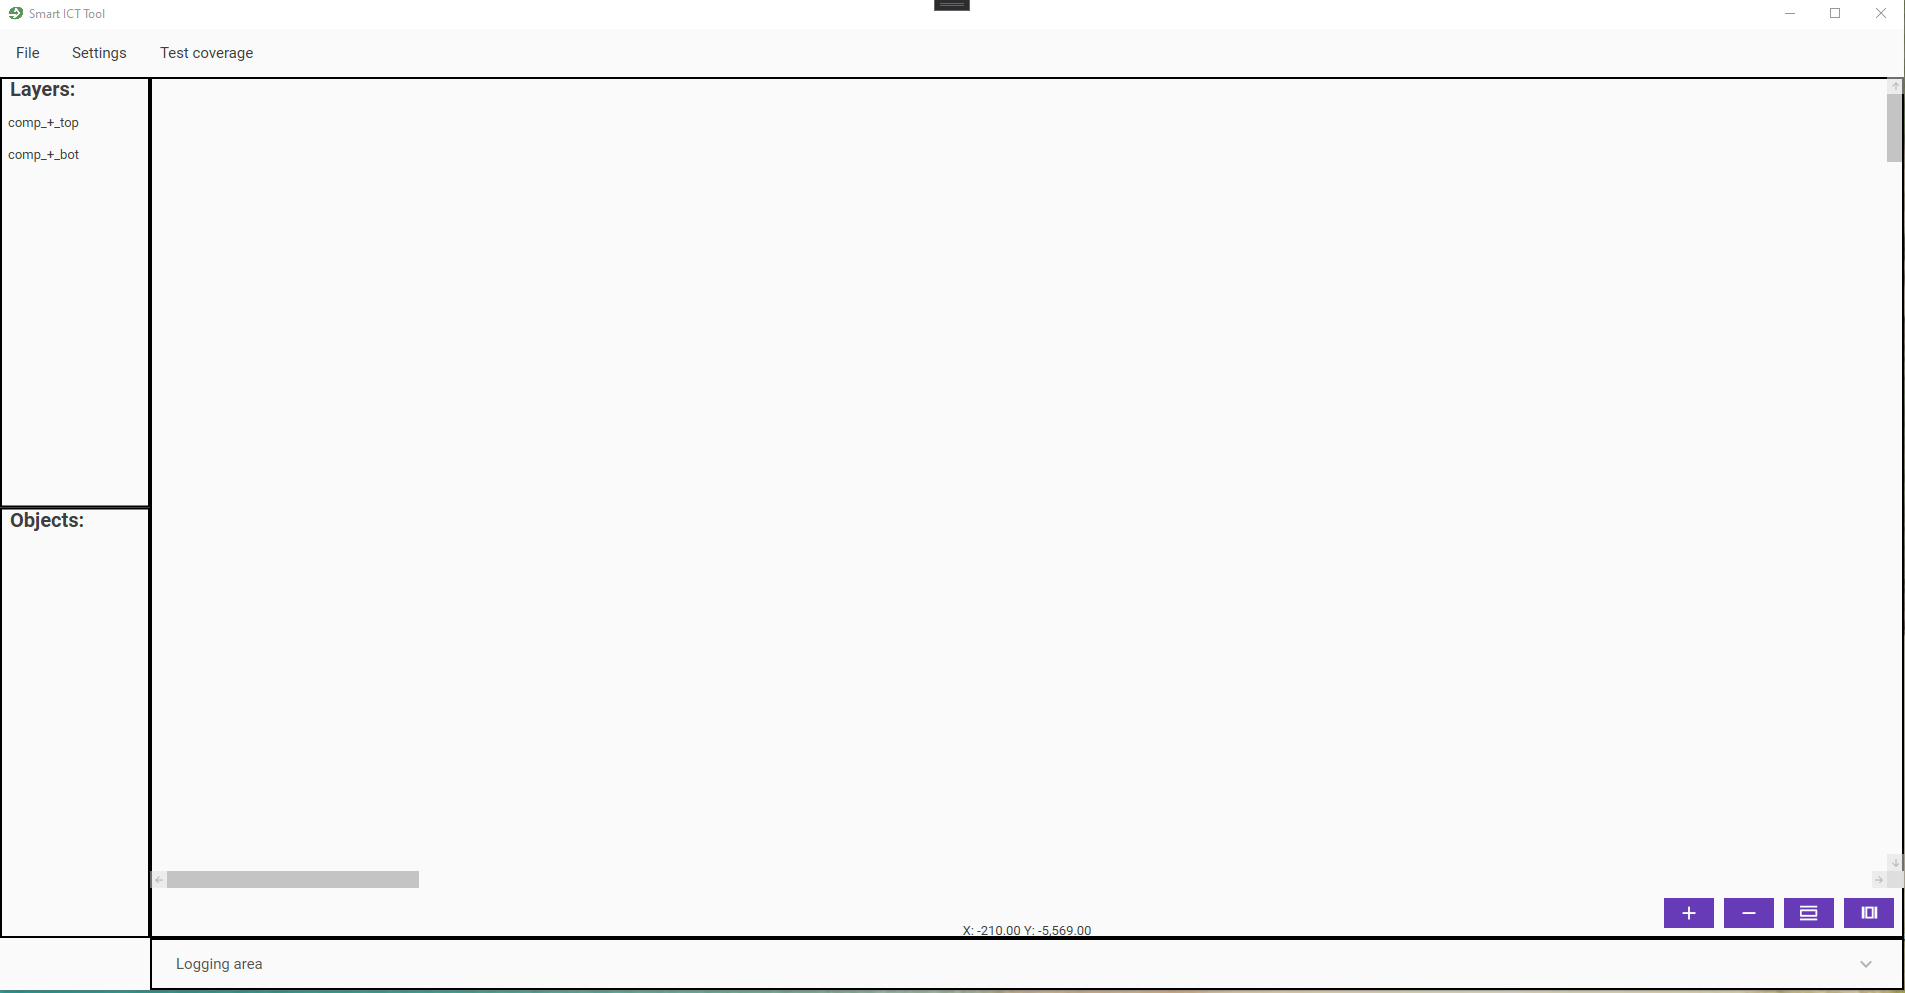
\includegraphics[width=1.00\textwidth]{figures/attachments/loadedProject.png}
	\begin{figure}[!h]
	\caption{Loaded project view}
	\label{fig:loadedProject}
	\end{figure}
\end{center}

After selecting for example the first layer then all components which are included within that layer should be rendered within the component view.

\begin{center}
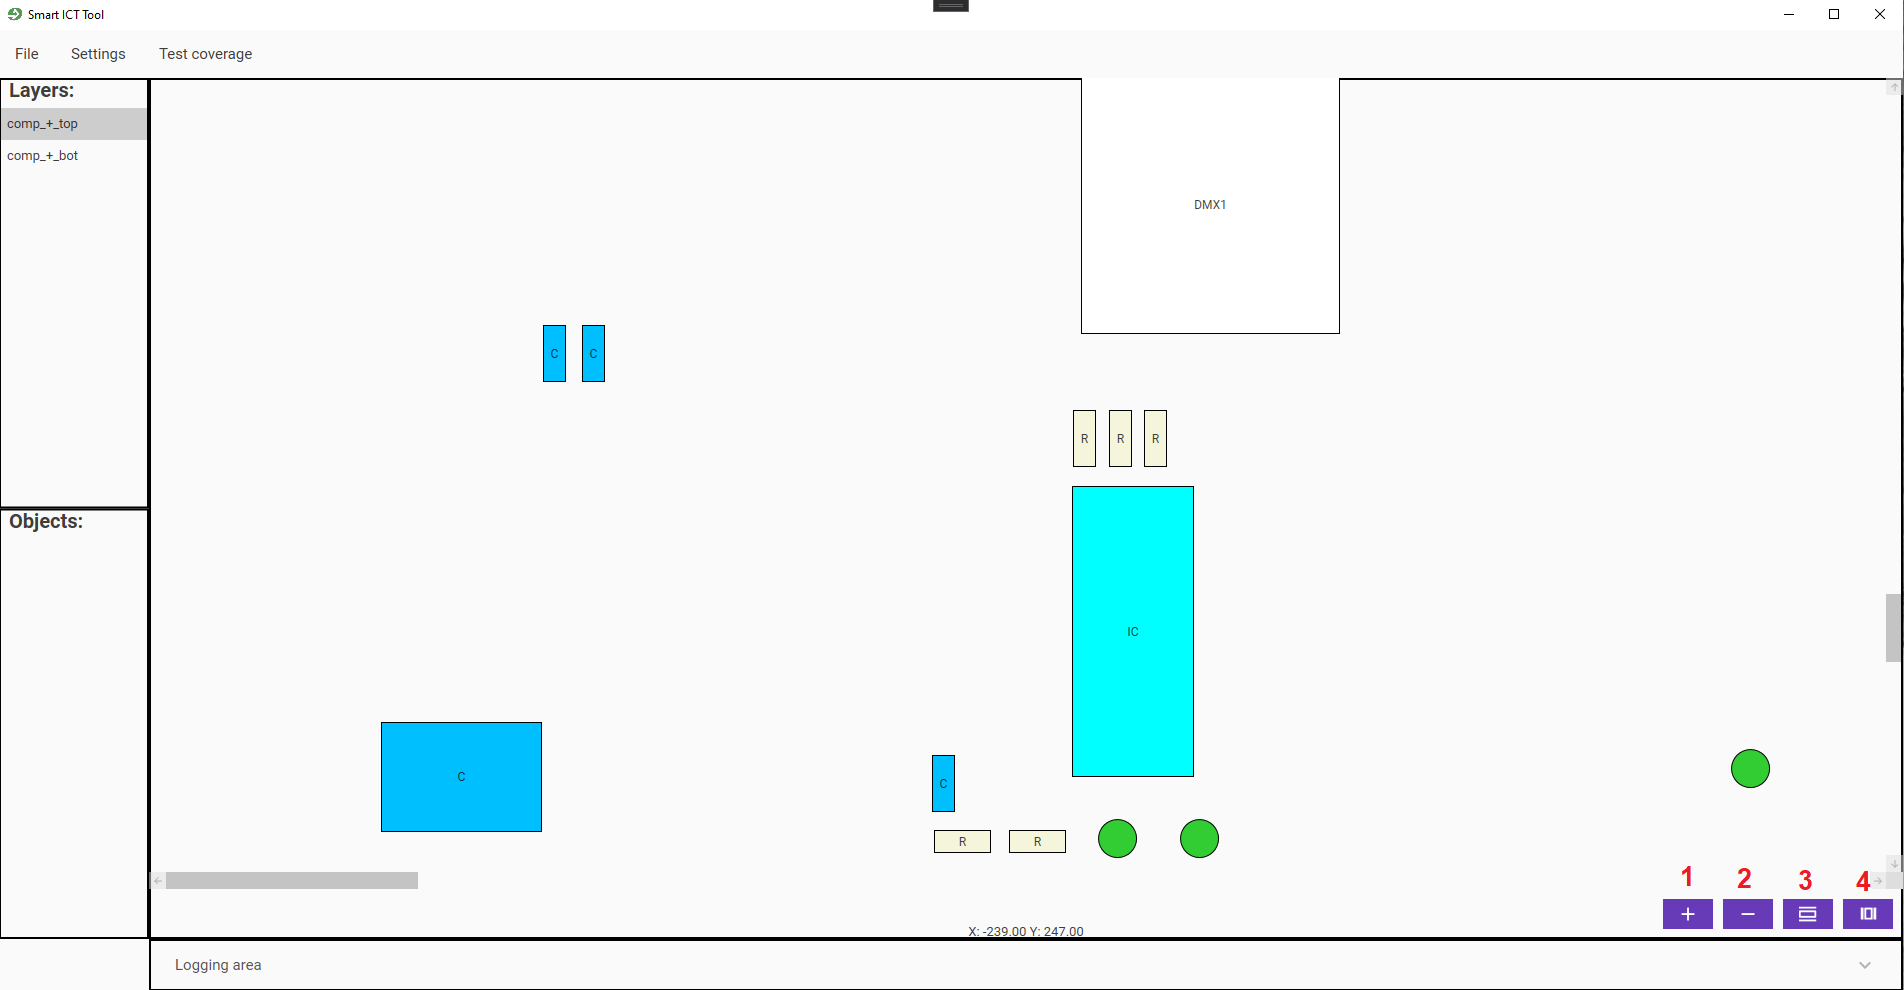
\includegraphics[width=1.00\textwidth]{figures/attachments/layerSelected.png}
	\begin{figure}[!h]
	\caption{Compontens view for selected layer}
	\label{fig:layerSelected}
	\end{figure}
\end{center}

As shown in \ref{fig:layerSelected} there is the possibility of scrolling with the mouse to move the whole view or just by clicking and dragging the whole content. Further there is the possibility of zooming in by pressing STRG and scrolling in or just by clicking on the zoom in button \textbf{1} and to zoom out by pressing STRG and scrolling out with the mouse or just by clicking the zoom out button \textbf{2}. Finally there is the possibility to mirror the whole view across the y axis \textbf{3} and the x axis \textbf{4}. Now to ensure not to have to use the \ac{GRPC} server again the next time you will open this project click File -> Miscellaneous -> Export data into \ac{JSON} file. After you chose it a new dialog will appear where you could type in just the name as the file itself will be stored within the project 
file as you are working within the project file mode. (Also all other project related data was automatically saved in the project file). Finally you should also 
export your current made settings by Settings -> Export settings file to make sure that the settings file is also included in the project file for later loading

\section{Working with the components view}
By right clicking on any object within the components view there will be a context menu visible:

\begin{center}
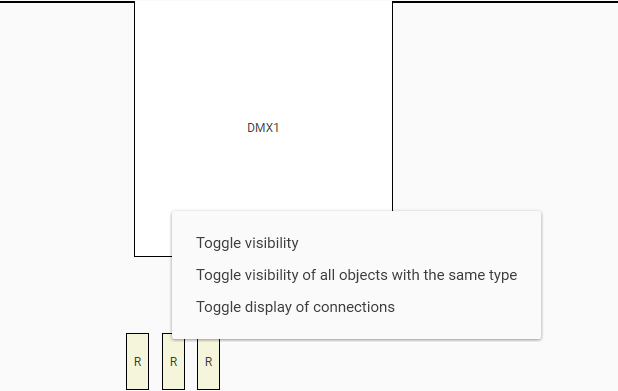
\includegraphics[scale=0.60]{figures/attachments/contextMenu.png}
	\begin{figure}[!h]
	\caption{Context menu of right click on component}
	\label{fig:contextMenu}
	\end{figure}
\end{center}

As shown at \ref{fig:contextMenu} you have the possibility of:
\begin{itemize}
	\item Toggle visibility - if clicked then the according components transparency will be set to high
	\item Toggle visibility of all objects with the same type - if clicked then all the according components which have the same type as the selected ones transparency will be set to high
	\item Toggle display of connections - if clicked then all connections of the component will be shown as plain lines
\end{itemize}

\subsection{Toggle visibility}

\begin{center}
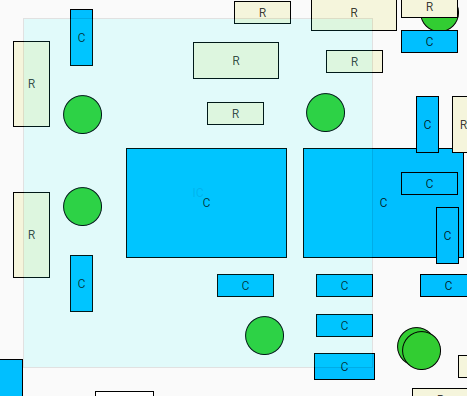
\includegraphics[scale=0.60]{figures/attachments/toggleVis.png}
	\begin{figure}[!h]
	\caption{Toggle visibility}
	\label{fig:toggleVis}
	\end{figure}
\end{center}

As shown in \ref{fig:toggleVis} after the visibility was toggled then the underlining objects could be determined

\subsection{Toggle visibility of all objects with the same type}

\begin{center}
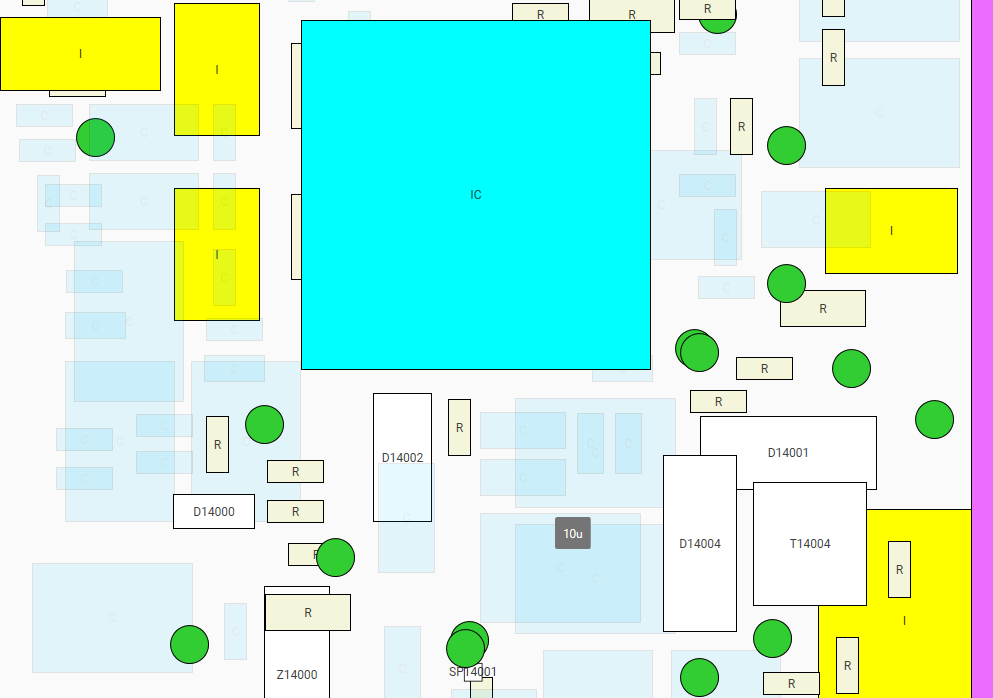
\includegraphics[scale=0.60]{figures/attachments/toggleVisAll.png}
	\begin{figure}[!h]
	\caption{Toggle visibility of all objects with the same type}
	\label{fig:toggleVisAll}
	\end{figure}
\end{center}

As shown in \ref{fig:toggleVis} after the visibility was toggled then the underlining objects of all toggled objects of the same type could be determined

\subsection{Toggle display of connections}

\begin{center}
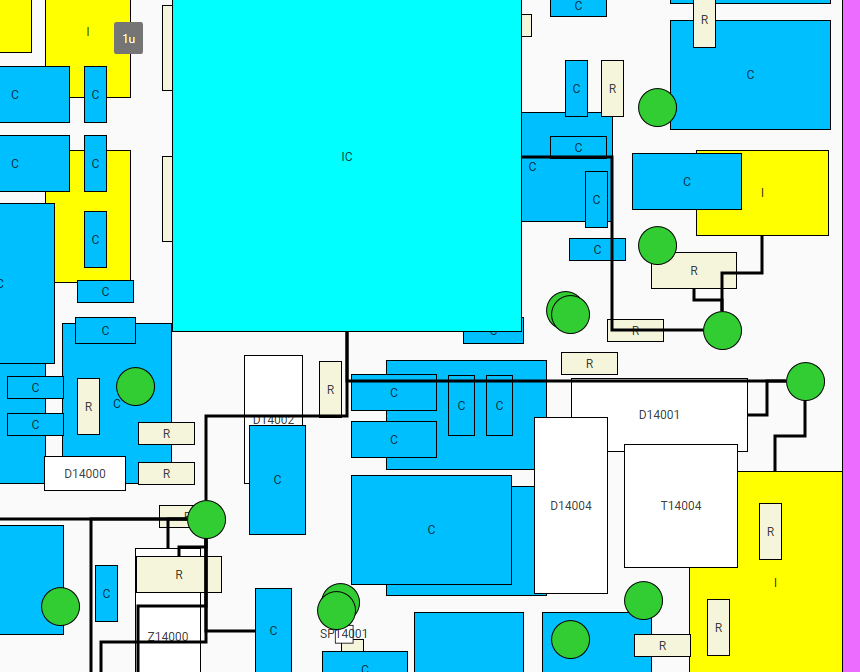
\includegraphics[scale=0.60]{figures/attachments/toggleConnection.png}
	\begin{figure}[!h]
	\caption{Toggle display of connections}
	\label{fig:toggleConnection}
	\end{figure}
\end{center}

As shown in \ref{fig:toggleConnection} after the connections were toggled then all lines will be drawn between the connecting objects.
Further there is the possibility to hover over any connection to see the following information:

\begin{center}
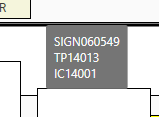
\includegraphics[scale=0.60]{figures/attachments/connectionLegend.png}
	\begin{figure}[!h]
	\caption{Legend of connection}
	\label{fig:connectionLegend}
	\end{figure}
\end{center}

As shown in \ref{fig:connectionLegend} there will be the following information available:

\begin{itemize}
	\item Net name
	\item Selected component for toggling the connections
	\item Connected component by this line to the selected component
\end{itemize}

\section{Test coverage}

\begin{center}
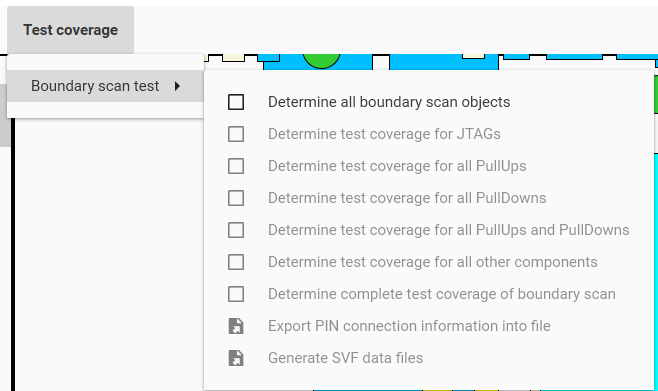
\includegraphics[scale=0.60]{figures/attachments/testCoverage.png}
	\begin{figure}[!h]
	\caption{Test coverage menu group}
	\label{fig:testCoverage}
	\end{figure}
\end{center}

As shown in \ref{fig:testCoverage} within the Test coverage -> Boundary scan test -> menu group there are the following menu items available:
\begin{itemize}
	\item Determine all boundary scan objects - before being able to perform any other test related action you have first to choose this one. (Settings will be considered)
	\item Determine test coverage for \ac{JTAG}s
	\item Determine test coverage for all PullUps
	\item Determine test coverage for all PullDowns
	\item Determine test coverage for all PullUps and PullDowns
	\item Determine test coverage for all other components
	\item Determine complete test coverage of boundary scan
	\item Export PIN connection information into file
	\item Generate \ac{SVF} data files
\end{itemize}

\subsection{Determine all boundary scan objects}
After you selected Test coverage -> Boundary scan test -> Determine all boundary scan objects then the objects list should be filled with new selection possibilities:

\begin{center}
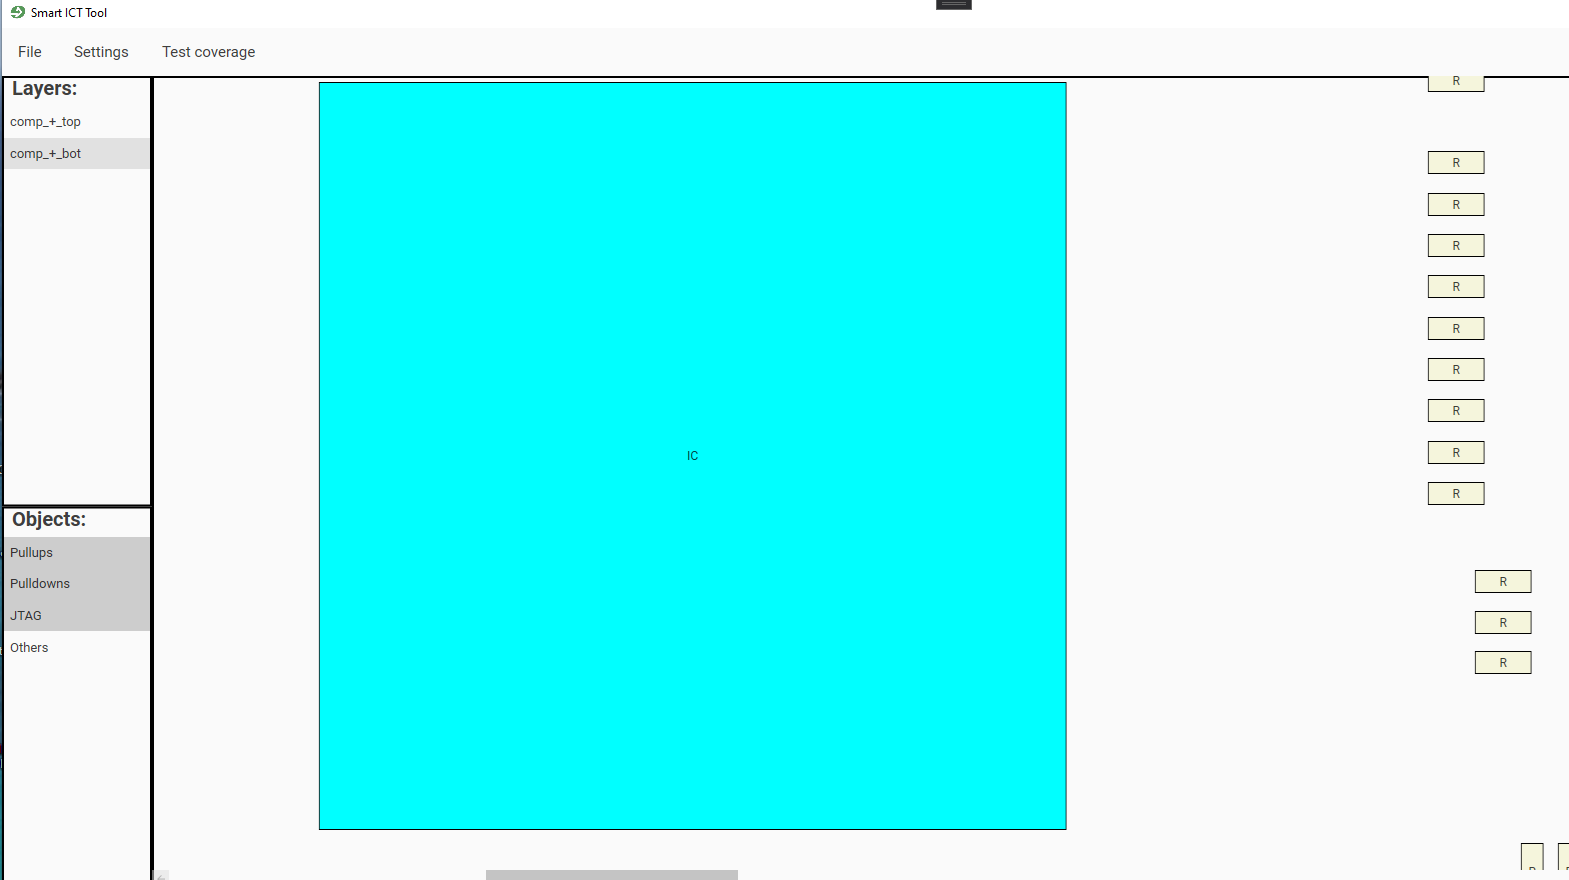
\includegraphics[width=1.00\textwidth]{figures/attachments/dterminedTestCoverageObjects.png}
	\begin{figure}[!h]
	\caption{Determine all boundary scan objects}
	\label{fig:dterminedTestCoverageObjects}
	\end{figure}
\end{center}

Now you could (\ref{fig:dterminedTestCoverageObjects}) select just the test coverage related objects of interest to be shown within the component view.

\subsection{Performing any test coverage of objects}

After you click for example on Test coverage -> Boundary scan test -> Determine test coverage for all PullUps then the calculated value will be shown as text and further more each connection to a according pull up resistor will be shown in green color:

\begin{center}
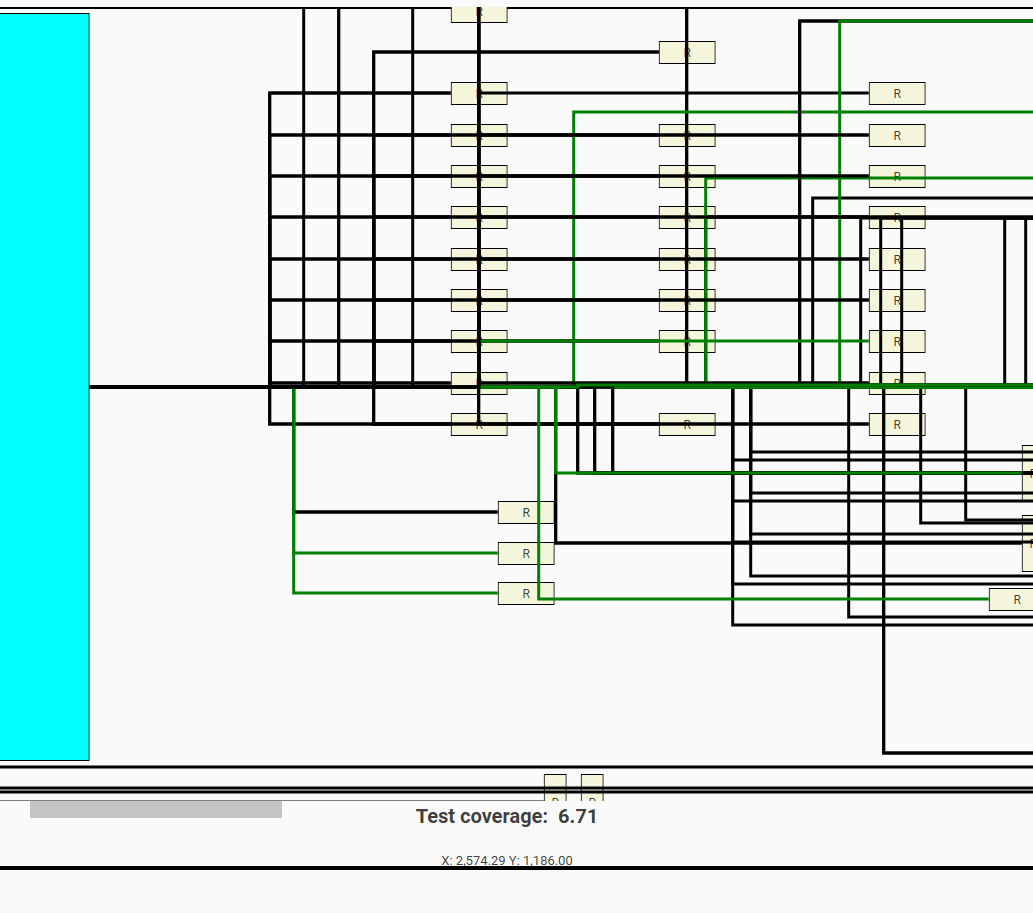
\includegraphics[width=1.00\textwidth]{figures/attachments/pullUpsTEstCoverage.png}
	\begin{figure}[!h]
	\caption{Determine test coverage for all PullUps}
	\label{fig:pullUpsTEstCoverage}
	\end{figure}
\end{center}

If you click again on Test coverage -> Boundary scan test -> Determine test coverage for all PullUps then the according check box will be unchecked and every connection is been showed just in black color again. This kind of procedure is also available for all other operations to detect the test coverage.

\subsection{Export PIN connection information into file}

After you click on Test coverage -> Boundary scan test -> Export PIN connection information into file a new dialog should appear where you can select the destination of file saving. After you selected that then the according file should be generate containing all pin information of interest of all \ac{JTAG} devices of the loaded project.

\subsection{Generate SVF data files}
If you click on Test coverage -> Boundary scan test -> Generate \ac{SVF} data files then first a dialog will be shown to select the target folder where to save the created files at. This folder will only be considered if you are not working in the project file mode. If so the files will be automatically been saved within the project file. Afterward you will be asked for selecting the according \ac{BSDL} file for all \ac{JTAG} devices found. After you selected the \ac{BSDL} file you will be informed about to make sure that the programmer is correctly connected to the \ac{JTAG} device as the default vector first needs to be read out:

\begin{center}
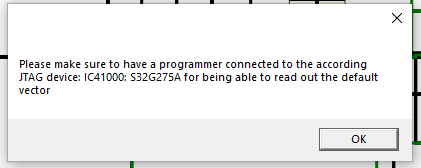
\includegraphics[scale=0.60]{figures/attachments/makeSureToConnect.png}
	\begin{figure}[!h]
	\caption{Make sure to have a programmer connected}
	\label{fig:makeSureToConnect}
	\end{figure}
\end{center}

After you confirmed the dialog \ref{fig:makeSureToConnect} then the read out will be performed and the according \ac{SVF} files for playing the pull down and pull up resistors will be generated.

\section{Log panel}

By clicking on the expander which is located at the very bottom of the application the log panel will be visible. It contains every single message logged during the working with the tool:

\begin{center}
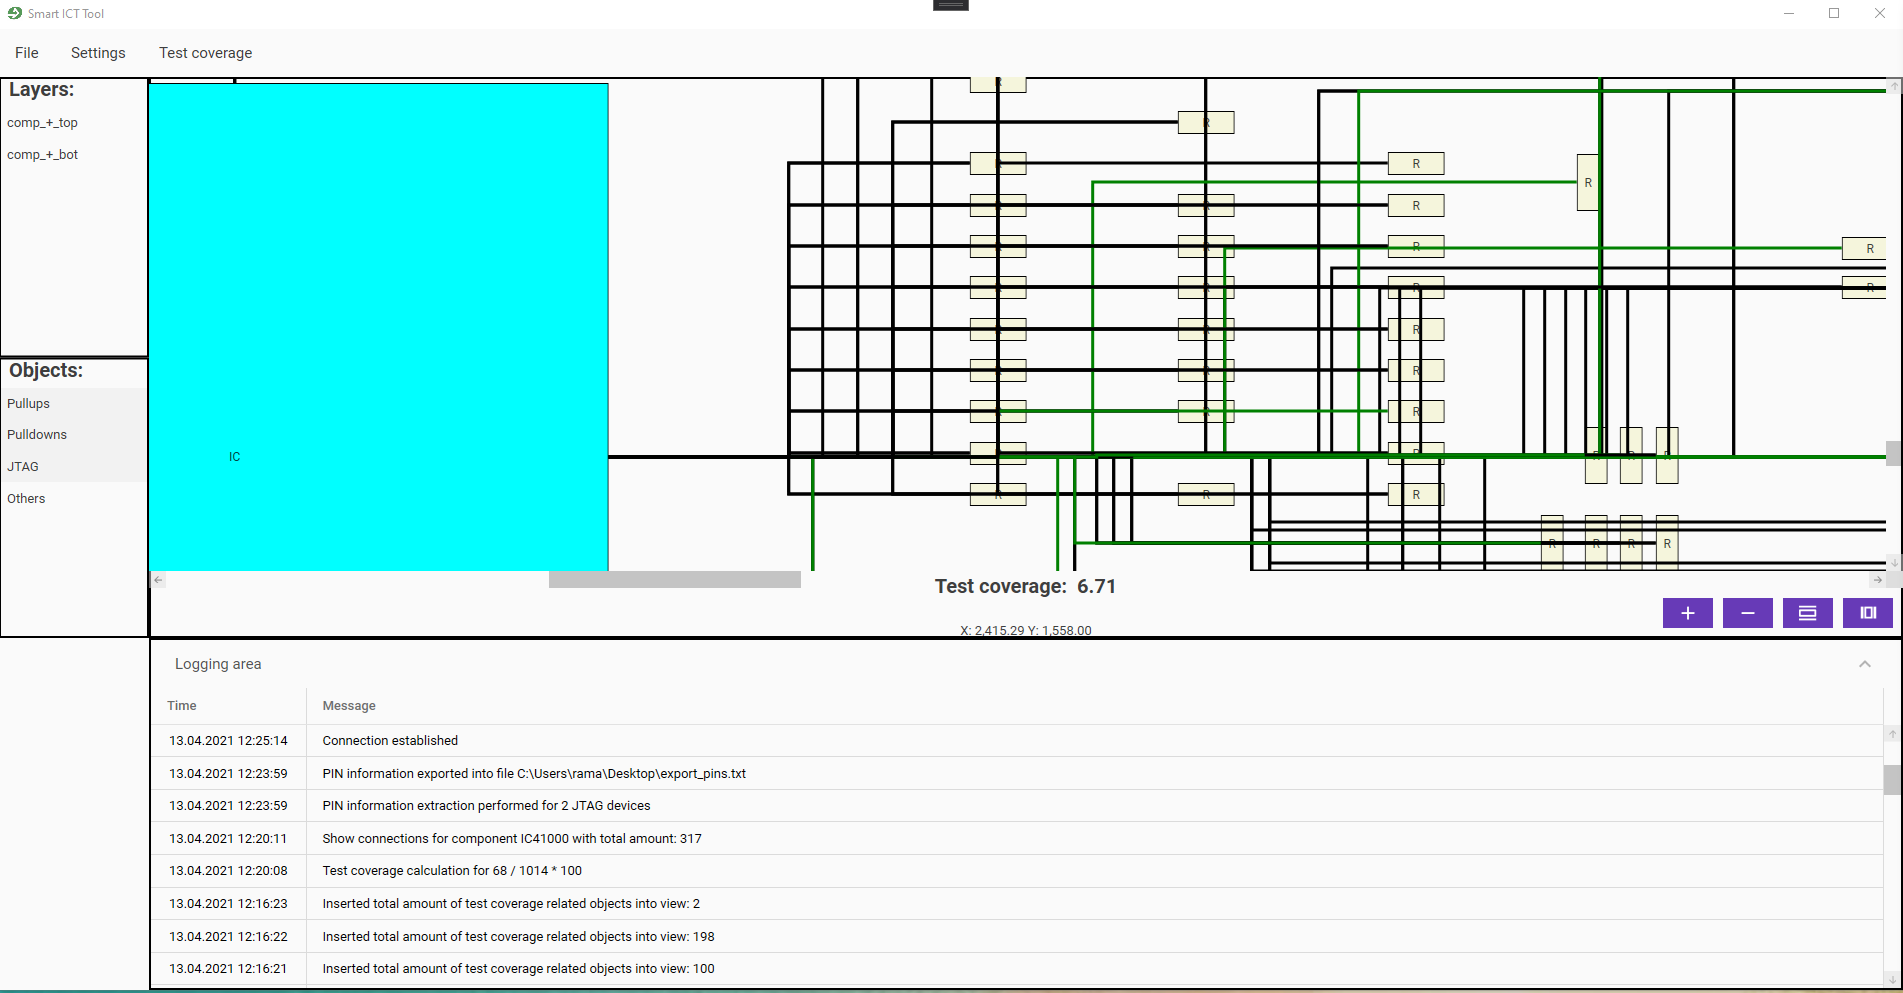
\includegraphics[width=1.00\textwidth]{figures/attachments/logging.png}
	\begin{figure}[!h]
	\caption{Logging area}
	\label{fig:logging}
	\end{figure}
\end{center}

\section{Drag and drop within the application}
You are further able to drag and drop directly files or folders to the application area. If something valid was dropped then it automatically should be opened or imported and if project mode is enabled saved further within the project file

\backmatter
\listoffigures

\listoftables

\renewcommand{\lstlistlistingname}{List of Listings}  % change for German thesis
\lstlistoflistings

\bibliographystyle{IEEEtran}
\bibliography{refs}
%\printnoidxglossaries

\end{document}
